\documentclass{article}
\usepackage[utf8]{inputenc}
\usepackage{helvet}
\usepackage{tikz}
% \usetikzlibrary{graphs, graphdrawing}
% \usegdlibrary{layered}
\usepackage{amsmath}

\title{Trees}
\date{\today}

\begin{document}

\maketitle

\paragraph{
  In computer science, trees are usually represented upside down. Trees can be used to represent an organization's structure showing the relationship between its different departments and their respective ranks and positions. Trees can also be used to represent file structures making it easy to locate the contents of the file. Trees can be used to represent a version control system where the repository of the project is stored on a centralized server with numerous programmers working on the copies of the project on their workstations.
}

\paragraph{
  Trees are specifically useful in computer science for their application in a wide range of algorithms.
}


\begin{itemize}
  \item Trees can be used to find the shortest path in a graph.
  \item Trees can be used in games such as checkers and chess and can help determine winning strategies.
  \item Trees can be used to model procedures carried out using a sequence of decisions.
  \item The concept of a binary tree is a fundamental data structure in high-level programming.
\end{itemize}

\section{Definition of a tree}

\title{Outlines}

\begin{itemize}
  \item Acyclic graphs
  \item Definition of a tree
  \item Definition of a forest
  \item Theorems on trees
  \item Definition of rooted trees
\end{itemize}

\subsection{Acyclic graphs}
\title{Definition}

\text{A graph G is called an acyclic graph if and only if G has no cycles.} \\

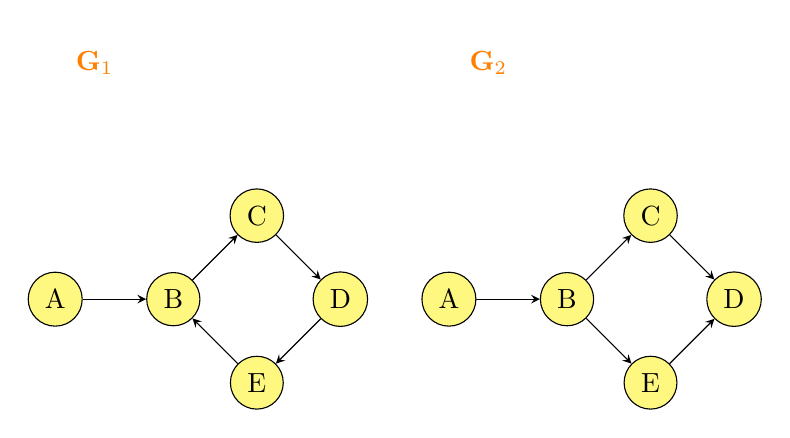
\begin{tikzpicture}
  [>=stealth, node distance=1.5cm, every node/.style={circle, draw, fill=yellow!50}]
  \begin{scope}[shift={(0,0)}]
  % \draw (1, -1) -- +(0,0) node[anchor=north] {G1};

  \node (A) {A};
  \node (B) [right of=A] {B};
  \node (C) [above right of=B] {C};
  \node (D) [below right of=C] {D};
  \node (E) [below right of=B] {E};
  
  \draw[->] (A) -- (B);
  \draw[->] (B) -- (C);
  \draw[->] (C) -- (D);
  \draw[<-] (B) -- (E);
  \draw[<-] (E) -- (D);
  \node[draw, white] at (0.5, 3) {\textcolor{orange}{\textbf{G$_1$}}};
  \end{scope}

  \begin{scope}[shift={(5,0)}]
    % \draw (1, -1) -- +(0,0) node[anchor=north] {G2};
  \node (A) {A};
  \node (B) [right of=A] {B};
  \node (C) [above right of=B] {C};
  \node (D) [below right of=C] {D};
  \node (E) [below right of=B] {E};
  
  \draw[->] (A) -- (B);
  \draw[->] (B) -- (C);
  \draw[->] (C) -- (D);
  \draw[->] (B) -- (E);
  \draw[->] (E) -- (D);
  \node[draw, white] at (0.5, 3) {\textcolor{orange}{\textbf{G$_2$}}};
  \end{scope}

\end{tikzpicture}

\paragraph{The directed graph G1 above, contains one cycle BCDEB, hence it is not an acyclic graph whereas G2 does not have any cycle in it. Thus G2 is an acyclic graph.}


\subsection{Definition of a tree}

\textbf{A tree is a connected acyclic undirected graph}
\paragraph{An undirected graph G is a tree if and only if it is connected and acyclic. This means that there exists a path between any two certices of G and G is cycle-free. Hence, a tree can have neither loops nor multiple edges (parallel edges). }


\begin{center}
  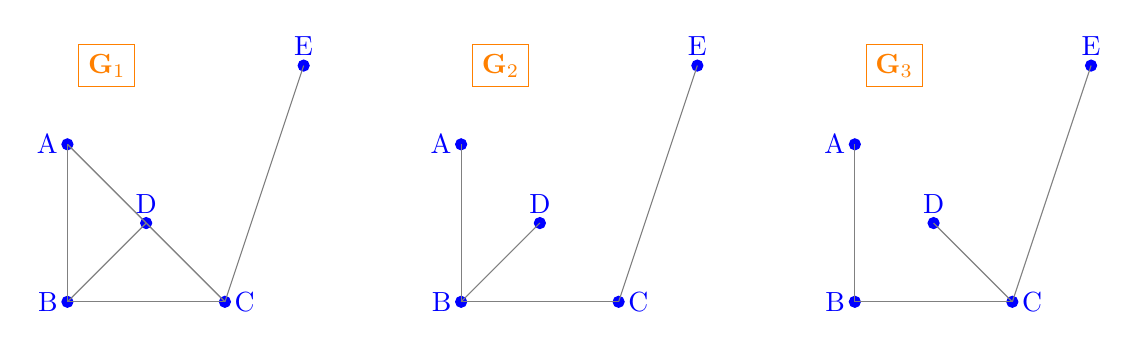
\begin{tikzpicture}
    \begin{scope}[shift={(0,0)}]
  % Draw the vertices
  \filldraw[blue] (0,2) circle (2pt) node[anchor=east] {A};
  \filldraw[blue] (0,0) circle (2pt) node[anchor=east] {B};
  \filldraw[blue] (2,0) circle (2pt) node[anchor=west] {C};
  \filldraw[blue] (1,1) circle (2pt) node[anchor=south] {D};
  \filldraw[blue] (3,3) circle (2pt) node[anchor=south] {E};
  
  % Draw the edges
  \draw[gray] (0,2) -- (0,0);
  \draw[gray] (0,0) -- (2,0);
  \draw[gray] (2,0) -- (0,2);
  \draw[gray] (0,2) -- (1,1);
  \draw[gray] (0,0) -- (1,1);
  \draw[gray] (1,1) -- (2,0);
  \draw[gray] (3,3) -- (2,0);
  
  \node[draw, orange] at (0.5, 3) {\textcolor{orange}{\textbf{G$_1$}}};
  \end{scope}

  \begin{scope}[shift={(5,0)}]
    % Draw the vertices
    \filldraw[blue] (0,2) circle (2pt) node[anchor=east] {A};
    \filldraw[blue] (0,0) circle (2pt) node[anchor=east] {B};
    \filldraw[blue] (2,0) circle (2pt) node[anchor=west] {C};
    \filldraw[blue] (1,1) circle (2pt) node[anchor=south] {D};
    \filldraw[blue] (3,3) circle (2pt) node[anchor=south] {E};
    
    % Draw the edges
    \draw[gray] (0,2) -- (0,0);
    \draw[gray] (0,0) -- (2,0);
    % \draw[gray] (2,0) -- (0,2);
    % \draw[gray] (0,2) -- (1,1);
    \draw[gray] (0,0) -- (1,1);
    % \draw[gray] (1,1) -- (2,0);
    \draw[gray] (3,3) -- (2,0);
    
    \node[draw, orange] at (0.5, 3) {\textcolor{orange}{\textbf{G$_2$}}};
  \end{scope}

  \begin{scope}[shift={(10,0)}]
    % Draw the vertices
    \filldraw[blue] (0,2) circle (2pt) node[anchor=east] {A};
    \filldraw[blue] (0,0) circle (2pt) node[anchor=east] {B};
    \filldraw[blue] (2,0) circle (2pt) node[anchor=west] {C};
    \filldraw[blue] (1,1) circle (2pt) node[anchor=south] {D};
    \filldraw[blue] (3,3) circle (2pt) node[anchor=south] {E};
    
    % Draw the edges
    \draw[gray] (0,2) -- (0,0);
    \draw[gray] (0,0) -- (2,0);
    % \draw[gray] (2,0) -- (0,2);
    % \draw[gray] (0,2) -- (1,1);
    % \draw[gray] (0,0) -- (1,1);
    \draw[gray] (1,1) -- (2,0);
    \draw[gray] (3,3) -- (2,0);
    
    \node[draw, orange] at (0.5, 3) {\textcolor{orange}{\textbf{G$_3$}}};
    \end{scope}
  
\end{tikzpicture}
\end{center}

\paragraph{The graph G1 above is a tree since it is connected but contains a cycle ABDA. The graph G2 is a tree since it is connected and has no cycles. The graph G3 is also a tree since it is connected cycle free.}

\subsection{Definition of a forest}

\paragraph{A forest is a collection of disjoint trees. A forest in nature contains many trees. A cycle-free disconnected graph is called a forest. The graph F below is a forest as it is disconnected and has no cycles. }

\begin{center}
  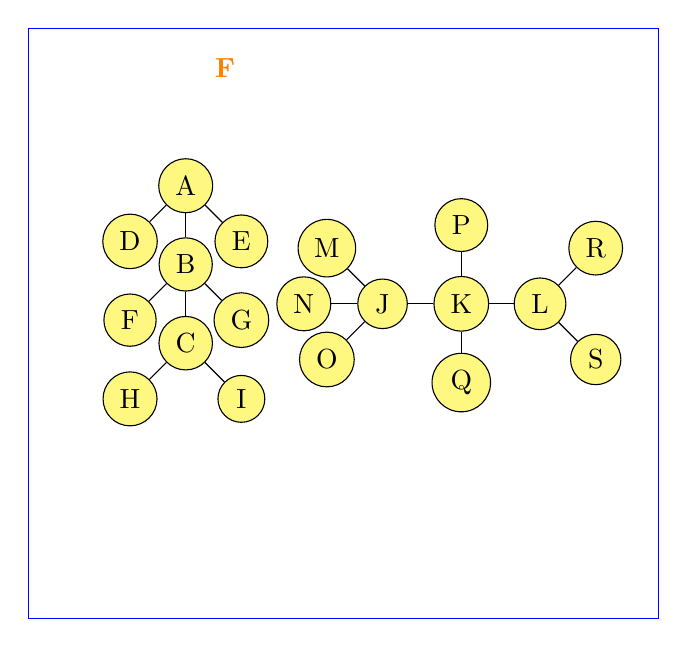
\begin{tikzpicture}
    [>=stealth, node distance=1cm, every node/.style={circle, draw, fill=yellow!50}]
  \begin{scope}[shift={(0,1.5)}]

  \node (A) {A};
  \node (B) [below of=A] {B};
  \node (D) [below left of=A] {D};
  \node (E) [below right of=A] {E};
  \node (C) [below of=B] {C};
  \node (F) [below left of=B] {F};
  \node (G) [below right of=B] {G};
  \node (H) [below left of=C] {H};
  \node (I) [below right of=C] {I};
  
  \draw[-] (A) -- (B);
  \draw[-] (B) -- (C);
  \draw[-] (A) -- (D);
  \draw[-] (B) -- (F);
  \draw[-] (B) -- (G);
  \draw[-] (A) -- (E);
  \draw[-] (C) -- (H);
  \draw[-] (C) -- (I);
  \end{scope}

  \begin{scope}[shift={(2.5,0)}]
  \node (J) {J};
  \node (N) [left of=J] {N};
  \node (M) [above left of=J] {M};
  \node (O) [below left of=J] {O};
  \node (K) [right of=J] {K};
  \node (P) [above of=K] {P};
  \node (Q) [below of=K] {Q};
  \node (L) [right of=K] {L};
  \node (R) [above right of=L] {R};
  \node (S) [below right of=L] {S};

  \draw[-] (J) -- (N);
  \draw[-] (J) -- (M);
  \draw[-] (J) -- (O);
  \draw[-] (J) -- (K);
  \draw[-] (K) -- (P);
  \draw[-] (K) -- (Q);
  \draw[-] (K) -- (L);
  \draw[-] (L) -- (R);
  \draw[-] (L) -- (S);
  
  \end{scope}
  \draw[blue] (-2, -4) rectangle (6, 3.5);
  \node[draw, white] at (0.5, 3) {\textcolor{orange}{\textbf{F}}};
  \end{tikzpicture}
\end{center}

\subsection{Theorems on trees}

\subsubsection{Theorem 1}

\textbf{An undirected graph is a tree if and only if there is unique and simple path betweeen any two vertices of the graph.}

\paragraph{Proof by contradiction (also known as absurdum): Suppose there are two distinct paths between two vertices of a tree. Then there must be a cycle in the tree which contradicts the definition of a tree. Hence, there is a unique path between any two vertices of a tree.}

\begin{center}
  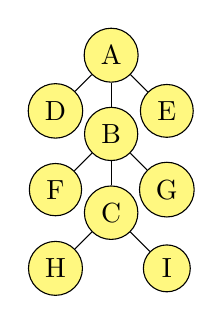
\begin{tikzpicture}
    [>=stealth, node distance=1cm, every node/.style={circle, draw, fill=yellow!50}]
  \begin{scope}[shift={(0,1.5)}]

  \node (A) {A};
  \node (B) [below of=A] {B};
  \node (D) [below left of=A] {D};
  \node (E) [below right of=A] {E};
  \node (C) [below of=B] {C};
  \node (F) [below left of=B] {F};
  \node (G) [below right of=B] {G};
  \node (H) [below left of=C] {H};
  \node (I) [below right of=C] {I};
  
  \draw[-] (A) -- (B);
  \draw[-] (B) -- (C);
  \draw[-] (A) -- (D);
  \draw[-] (B) -- (F);
  \draw[-] (B) -- (G);
  \draw[-] (A) -- (E);
  \draw[-] (C) -- (H);
  \draw[-] (C) -- (I);
  \end{scope}
  \end{tikzpicture}
\end{center}

\paragraph{Example: Given a graph G, let's assume that G is a tree, then G is connected and has no cycles. Let B and I be two vertices in G. We need to show there is a unique path between B and I. Let \(P_1\) be a path from B to I. Let's assume there is another path \(P_2\) between B and I. Hence we can combine the first part from B to I with the part from I to B obtained by reversing the order of the second path. The result will form a cycle which is a contradiction of the hyptothesis as the graph is a tree. Hence there exists a unique single path. }

\subsubsection{Theorem 2}

\textbf{A tree with n vertices has n-1 edges.}

\subsection{Definition of rooted trees}

\textbf{A rooted tree is a tree in which one vertex is designated as the root and every edge is directed away from the root.}


\section{Spanning trees of a graph}

\title{Outlines}
\begin{itemize}
  \item Spanning trees of a graph
  \item Constructing a spanning tree
  \item Non-isomorphic spanning trees of a graph
\end{itemize}

\subsection{Spanning trees of a graph}

\paragraph{In many real life problems such as internet multicasting and network routing, it is important to find a tree that connects all the vertices of a graph. This tree is called a spanning tree.}

\subsubsection{Definition}

\textbf{A spanning tree of a graph G is a connected subgraph of G that contains all the vertices of G but carries no cycles.}

\begin{center}
  \begin{tikzpicture}
    [>=stealth, node distance=1cm, every node/.style={circle, draw}]

    \begin{scope}[shift={(0,2)}]
      \node (A) {};
      \node (B) [below of = A] {};
      \node (C) [right of = B] {};
      \node (D) [right of = A] {};

      \draw[-] (A) -- (B);
      \draw[-] (B) -- (C);
      \draw[-] (C) -- (D);
      \draw[-] (D) -- (A);
      \draw[-] (A) -- (C);
      \draw[-] (B) -- (D);
      
      \node[draw, white] at (0.5, 1) {\textcolor{orange}{\textbf{G}}};
    \end{scope}

    \begin{scope}[shift={(3,0)}]
      \node (A) {};
      \node (B) [below of = A] {};
      \node (C) [right of = B] {};
      \node (D) [right of = A] {};

      \draw[-] (A) -- (B);
      % \draw[-] (B) -- (C);
      \draw[-] (C) -- (D);
      \draw[-] (D) -- (A);
      % \draw[-] (A) -- (C);
      % \draw[-] (B) -- (D);
      
      \node[draw, white] at (3,4 ) {\textcolor{orange}{\textbf{T$_1$}}};
    \end{scope}

    \begin{scope}[shift={(3,1.5)}]
      \node (A) {};
      \node (B) [below of = A] {};
      \node (C) [right of = B] {};
      \node (D) [right of = A] {};

      \draw[-] (A) -- (B);
      % \draw[-] (B) -- (C);
      \draw[-] (C) -- (D);
      % \draw[-] (D) -- (A);
      \draw[-] (A) -- (C);
      % \draw[-] (B) -- (D);
      
      \node[draw, white] at (3, 1) {\textcolor{orange}{\textbf{T$_2$}}};
    \end{scope}

    \begin{scope}[shift={(3,3)}]
      \node (A) {};
      \node (B) [below of = A] {};
      \node (C) [right of = B] {};
      \node (D) [right of = A] {};

      \draw[-] (A) -- (B);
      \draw[-] (B) -- (C);
      % \draw[-] (C) -- (D);
      % \draw[-] (D) -- (A);
      % \draw[-] (A) -- (C);
      \draw[-] (B) -- (D);
      
      \node[draw, white] at (3, -2) {\textcolor{orange}{\textbf{T$_3$}}};
    \end{scope}

    \begin{scope}[shift={(3,4.5)}]
      \node (A) {};
      \node (B) [below of = A] {};
      \node (C) [right of = B] {};
      \node (D) [right of = A] {};

      % \draw[-] (A) -- (B);
      \draw[-] (B) -- (C);
      \draw[-] (C) -- (D);
      \draw[-] (D) -- (A);
      % \draw[-] (A) -- (C);
      % \draw[-] (B) -- (D);
      
      \node[draw, white] at (3, -5) {\textcolor{orange}{\textbf{T$_4$}}};
    \end{scope}
    \draw[blue] (-2, -2.5) rectangle (8, 5.5);
  \end{tikzpicture}
\end{center}

\subparagraph{The graph G above is a connected graph with no cycles. The graphs T$_1$, T$_2$, T$_3$ and T$_4$ are spanning trees of G.}

\subsection{Constructing a spanning tree}

\subsubsection{To get a spanning tree of a graph G}

\begin{itemize}
  \item Keep all vertices of G
  \item Break all the cycles but keep the tree connected
\end{itemize}

\subsection{Non-isomorphic spanning trees of a graph}

\subsubsection{isomorphic Spanning trees}

\textbf{Two spanning trees are said to be isomorphic if there is a bijection preserving adjacency between the two trees.}

\paragraph{Some of the spanning trees of a graph may be isomorphic which means they are the same. However, if we are asked to find all the spanning trees of a graph, we are only intersted in the non-isomorphic spanning trees. In the last example, the spanning trees T$_4$, T$_3$ and T$_1$ are isomorphic to each other, however, T$_4$, T$_3$ and T$_1$ are all non-isomorphic to T$_2$. So if we are asked to draw non-iomorphic trees of graph G, then we only need to draw T$_2$ and one of the rest of the the three non-isomorphic trees.}

\section{Minimum spanning tree}

\title{Outlines}

\begin{itemize}
  \item Example of a use
  \item Weight of a spanning tree
  \item Minimum spanning Trees
  \item Kruskal's algorithm
  \item Prim's algorithm
\end{itemize}

\textbf{Example of a use case}

\paragraph{Suppose we want to supply a set of houses with:}

\begin{itemize}
  \item electric power
  \item water pipes
  \item sewage lines
  \item telephone lines
\end{itemize}

\paragraph{To keep costs down, you could connect these houses with a spanning tree(power lines, for example). However, the houses are not all equal distances apart.}

\paragraph{To reduce costs even further, you could connect the houses with a minimum-cost spanning tree.}

\paragraph{Suppose you have a connected undirected graph with a weight (or cost) associated with each edge.}

\paragraph{The cost of a spanning tree would be the sum of the cost of its edges.}

\subsection{Minimum cost spanning tree}

\textbf{A minimmum cost spanning tree is a spanning tree that has the lowest weight (lowest cost).}

\subsection{Finding spanning trees}

\paragraph{There are two basic algortihms for finding minimum-cost spanning trees, and both are greedy algorithms:}

\begin{itemize}
  \item Kruskal's algorithm
  \item Prim's algorithm
\end{itemize}


\subsection{Kruskal's algorithm}

\paragraph{Start with the cheapest edges in the spanning tree}
\paragraph{Repeatedly add the cheapest edge that does not create a cycle}

\subsection{Prim's algorithm}

\paragraph{Start with any node in the spanning tree}
\paragraph{Repeatedly add the cheapest edge, and the node it leads to, for which the node is not already in the spanning tree.}


\end{document}
